\part*{Lecture 5: \\Simulation}

Suppose you flip a coin 100 times. The result of this process will be a sequence of 100 heads and tails, such as HTTHTHHH...HT. Let's define a `run of size n' to be a continuous sequence of $n$ heads or $n$ tails in a row. The example sequence above, for instance, begins with a run of size 1 (H), followed by one of size 2 (TT), followed by one of size 1 (H), and so on.

What do you think the longest run will be? What's the probability it's more than 8? This is the kind of problem that you wouldn't see in a math class, because --- like most real-world problems --- it's too hard to work out by hand.

With a computer, though, you can easily find a practical answer. Here's the idea. Using a random number generator (we'll use Python's \texttt{random} library), have the computer flip 100 coins in a row and compute the length of the longest run. Then have the computer do it a few more times--- say a hundred thousand more times. Then, if we wanted to find the probability that the longest run is longer than 8, we can just have the computer return the fraction of times the longest run was longer than 8. Here's code to do this below:

\begin{lstlisting}
import random

def flip_coins(n): 
	# Returns a string of n coin flips, like 'HTTHTHHH...HT'
	coin_tosses = ''
	for i in range(n):
		# random.choice() takes in a list and returns a random element from it
		coin_tosses += random.choice(['H', 'T']) 
	return coin_tosses

def compute_longest_run(coin_tosses): 
	# coin_tosses should be a string as output by flip_coins(). 
	# Returns the length of the longest run
	
	# The procedure is to scan through the string, counting each run length
	longest_run_length = 1
	current_index = 0
	current_run_length = 1
	while current_index <= len(coin_tosses) - 2:
		# If next letter is the same, increment current run length
		if coin_tosses[current_index + 1] == coin_tosses[current_index]: 
			current_run_length += 1
			if current_run_length > longest_run_length:
				longest_run_length = current_run_length
		else:
			current_run_length = 1
		current_index += 1
	return longest_run_length

def collect_longest_run_data(coin_flips_per_trial,num_trials): 
	'''
	returns an array of length coin_flips_per_trial, where the element 
	at index i is the number of times the longest run was of length i+1.
	'''	
	output_array = coin_flips_per_trial * [0]
	for i in range(num_trials):
		coin_toss_sequence = flip_coins(coin_flips_per_trial)
		longest_run = compute_longest_run(coss_toss_sequence)
		output_array[longest_run - 1] += 1
	return output_array
\end{lstlisting}

Let's save the above as \texttt{coin\_toss.py}. We'll now use it as a library to find the probability that the longest run will be at least 8.

\begin{lstlisting}
import coin_toss

TRIALS = 100000 # One hundred thousand trials!
longest_run_data = coin_toss.collect_longest_run_data(100, TRIALS)
# And count up the number of times it was more than 8...
trials_more_than_8 = 0
for i in range(7,100):
        trials_more_than_8 += longest_run_data[i]
fraction_more_than_8 = trials_more_than_8 / TRIALS
print(fraction_more_than_8)
\end{lstlisting}

Running the program, we see the probability of having a run of at least 8 is $\sim$\texttt{.31}! 

Maybe you're more interested in knowing the probabilities that the longest run will be exactly 1, 2, 3, 4, ..., 100. Let's do that.

\begin{lstlisting}
import coin_toss

TRIALS = 100000
longest_run_data = coin_toss.collect_longest_run_data(100, TRIALS)
for i in range(100):
        run_length = i + 1
        fraction = longest_run_data[i] / TRIALS
        print('Chance longest run is of length ' + str(run_length) + 
        	  ': ' + str(fraction))
\end{lstlisting}

Running this will then print the desired probabilities:

\begin{lstlisting}[numbers=none]
Chance longest run is of length 1: 0.0
Chance longest run is of length 2: 0.0
Chance longest run is of length 3: 0.00031
Chance longest run is of length 4: 0.02722
Chance longest run is of length 5: 0.16408
Chance longest run is of length 6: 0.26483
Chance longest run is of length 7: 0.22826
Chance longest run is of length 8: 0.14805
Chance longest run is of length 9: 0.08138
...
Chance longest run is of length 100: 0.0
\end{lstlisting}

Seeing a big list of numbers isn't the best way to show the results to someone else, though. Wouldn't it be nicer to have a bar graph with run length on the x-axis and the probabilities represented by bar heights? 

There's a very popular library to build visualizations like this, \texttt{matplotlib}. Let's use it to build the bar plot we want:

\begin{lstlisting}
import coin_toss
import matplotlib.pyplot as plt 
# This just means we can use the shorter string plt instead 
# of matplotlib to refer to the library later in the program

TRIALS = 100000
longest_run_data = coin_toss.collect_longest_run_data(100, TRIALS)
fractions = []
for item in longest_run_data:
        fractions.append(item / TRIALS)
        
# Now we're going to build a plot using matplotlib's bar plot function. 
# The first parameter is the list of x-values, 
# and the second parameter is the list of heights.
plt.bar(list(range(1, 21)), fractions[:20])
# matplotlib plots also have functions to add titles and labels to make 
# your plot nice, let's use a few of those.
plt.xlabel('Longest Run Length')
plt.ylabel('Probability')
plt.title('Longest Run Length when Flipping 100 Coins')
plt.show()
\end{lstlisting}

\begin{center}
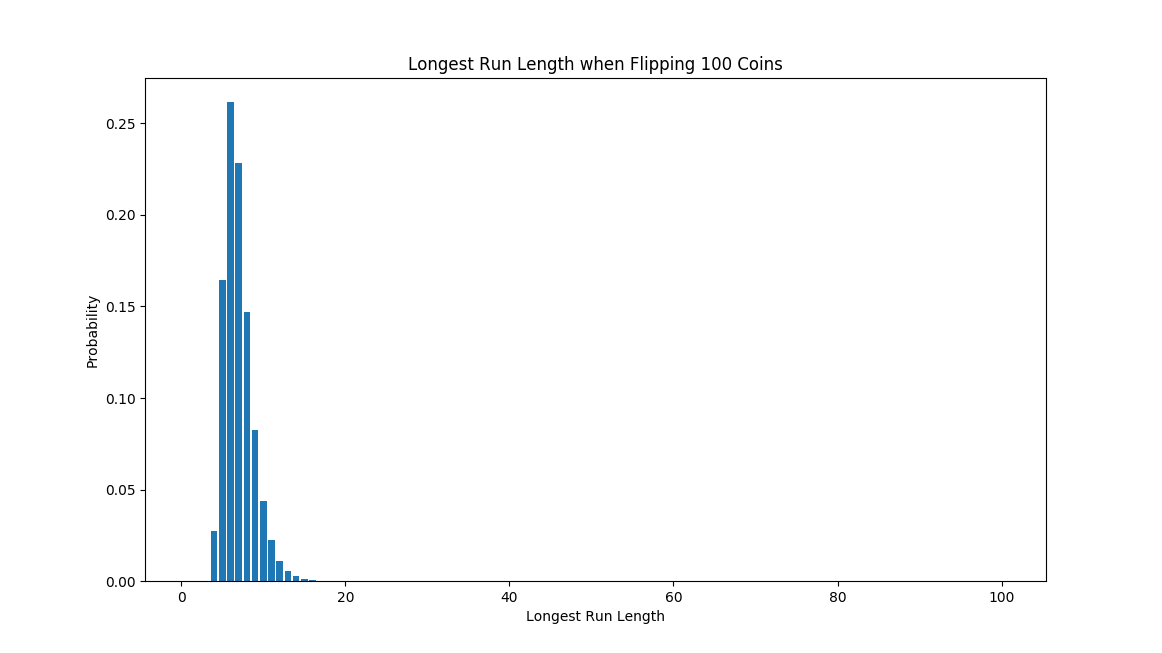
\includegraphics[width=13cm]{coin_plot_1}
\end{center}

We can also focus in on the interesting part of the plot by limiting the input to \texttt{plt.bar} to the first 20 elements of each array. This yields the following:

\begin{center}
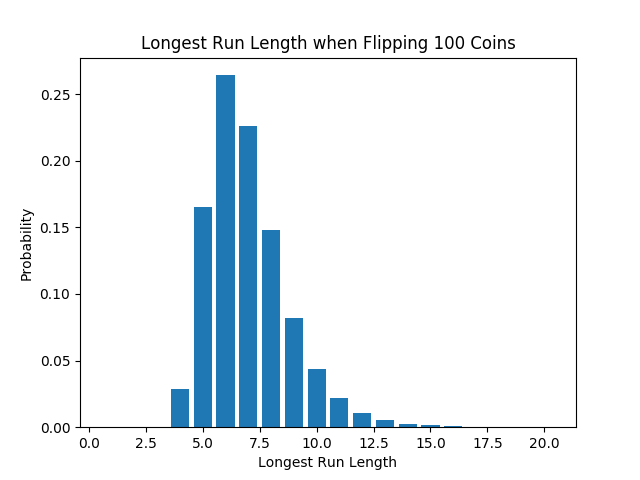
\includegraphics[width=13cm]{coin_plot_2}
\end{center}

Matplotlib provides the tools to build most any kind of plot you might be interested in. It also has many more functions to give you careful control over the resulting plot (for example, to fix the x-values in the above plot to be whole numbers). You can learn more and read the documentation at their website, matplotlib.org.
